\documentclass[11pt,twocolumn,a4paper,DIV=calc,parskip=half]{scrartcl}
\usepackage[protrusion=true,expansion=true]{microtype}
\usepackage[utf8]{inputenc}
\usepackage[T1]{fontenc}
\usepackage{graphicx}
\usepackage{hyperref}
\usepackage{mathptmx}
\usepackage[scaled=.92]{helvet}
\usepackage{booktabs}
\usepackage{amsmath, amsthm}
\newtheorem{theorem}{Theorem}
\newtheorem{definition}{Definition}
\usepackage{amssymb}
\usepackage{enumitem}
\usepackage{xcolor}
\usepackage{multirow}
\usepackage{subcaption}
\usepackage{tikz}
\usepackage{pgfplots}
\usepackage[table,xcdraw]{xcolor}
\pgfplotsset{compat=1.18}
\usepackage[printonlyused]{acronym}

% --------------------------------------------------
% Placeholder command
% --------------------------------------------------
\newcommand{\placeholder}[1]{\textcolor{gray}{\textit{[#1]}}}

\begin{document}
	
	% --------------------------------------------------
	% Front Matter
	% --------------------------------------------------
	\title{Navigating the Privacy--Robustness--Performance Trilemma in Federated Learning}
	\author{Jonas Müller \and Rebekka Schnoor}
	\date{\today}
	\maketitle
	
	\begin{abstract}
		\placeholder{%
			2--4 sentences summarizing the paper: motivation (the trilemma), what we did
			(8-configuration empirical study on MNIST/CIFAR-10 with Flower+Opacus+BLADES),
			key finding (compounding behavior, direction of magnitude), and main take-away
			for practitioners.%
		}
	\end{abstract}
	
	\tableofcontents
	
	\section*{List of abbreviations}
	\begin{acronym}
		\acro{FL}{Federated Learning}
		\acro{IID}{independent and identically distributed}
		\acro{DP-SGD}{Differentially Private Stochastic Gradient Descent}
		\acro{SGD}{Stochastic Gradient Descend}
		\acro{DP}{Differential Privacy}
	\end{acronym}
	
% --------------------------------------------------
	\section{Introduction}
	% --------------------------------------------------
	
	We present a systematic empirical study of the Privacy--Robustness--Performance
	trilemma in \ac{FL}, examining how simultaneously deployed defenses
	interact and compound across all three axes.
	
	\placeholder{%
		Summarize results and contributions.%
	}
	
	\subsection{Background and Motivation}
	
	In the past ten years, \ac{FL} has emerged as a framework for achieving distributed training without the need for data centralization. This is of particular interest when processing sensitive data, such as in healthcare or mobile applications. The local training allows to leave the data with the clients but opens new attack surfaces for model poisoning during training through the transmission of manipulated updates. Also, the transmitted gradients can still leak information about the used training data set. Additionally, gradient transmission at each round causes significant communication cost, especially for complex models.
	
	In an effort to fortify the resilience of models and safeguard client privacy, numerous methodologies have been implemented in recent years. 
	Robustness-enhancing methods are designed to detect malicious updates by assuming a significant deviation from the honest majority. 
	Privacy-preserving algorithms add a mask or calibrated noise to the local updates before transmitting them to the central server.
	
	\subsection{Problem Statement}
	
	Ensuring model robustness and client privacy while balancing communication cost and model accuracy has been identified as a significant challenge.
	Adding privacy-enhancing noise to individual updates reduces a malicious server's ability to extract information about local datasets, while simultaneously reducing model accuracy.
	Discarding unusual updates improves robustness against Byzantine adversaries but risks disregarding legitimate updates, particularly in settings where data is not \ac{IID}.
	Compression techniques that reduce transmission load limit the information transmitted to the server and thus reduce model accuracy.
	
	In 2023, Allouah et al.~\cite{allouah2023trilemma} proved Theorem \ref{theorem:lowerBound}, stating that the combination of such methods yields a lower bound for the expected training error that exceeds the sum of the individual cost for robustness and privacy by a multiplicative term.
	\begin{theorem}
		Consider distributed mean estimation in $\mathbb{R}^d$ with $n$ users, of which an $\eta$-fraction may behave maliciously. Any algorithm, producing an estimate $\hat{\mu}$ of the true mean $\mu\in\mathbb{R}^d$ of inputs, and achieving $(\varepsilon,\delta)$-local \ac{DP} and robustness to $\eta$-corruption must incur an estimated error
		\begin{equation}
			\mathbb{E}\parallel \hat{\mu}-\mu\parallel _{2}^{2} = \tilde{\Omega}(\frac{\eta}{\varepsilon^{2}}+\frac{d}{\varepsilon^{2}n}+\eta G^{2}).
		\end{equation}
		\label{theorem:lowerBound}
	\end{theorem}
	
	A position paper by the same group~\cite{allouah2023balancing} highlights a gap between the theoretical lower bound and current
	implementations. 
	
	\subsection{Research Questions}
	
	The project is structured around three research questions:
	\begin{enumerate}
		\item \textbf{Isolation:} What is the individual cost of each defense mechanism
		(\ac{DP}, Byzantine-robust aggregation, gradient compression) in terms of accuracy,
		communication overhead, and attack success rate, and do our results reproduce
		the published baselines?
		\item \textbf{Combination:} How do pairwise and full combinations of the three
		mechanisms interact? Do the costs compound additively, sub-additively, or
		super-additively?
		\item \textbf{Mitigation:} Can simple adjustments --- e.g.\ joint calibration of
		the \ac{DP} clipping norm and the robust aggregation threshold --- reduce the
		compounding effect without sacrificing formal guarantees?
	\end{enumerate}
	
	\subsection{Contributions}
	
	\placeholder{%
		Bullet list mirroring Section~6 of the Exposé:
		(i) systematic 8-configuration mapping on MNIST/CIFAR-10 with joint trilemma
		reporting;
		(ii) reproduction and cross-framework extension of BLADES baselines;
		(iii) initial test of joint clipping-norm calibration as a mitigation heuristic;
		(iv) open-source reproducible pipeline.%
	}
	
	\subsection{Structure of the Report}
	
	The remainder of the report is organized as follows.
	Section~\ref{sec:background} provides the theoretical background of all three
	trilemma axes and derives the joint lower bound.
	Section~\ref{sec:threat} defines the threat model and evaluation metrics.
	Section~\ref{sec:method} describes the chosen mechanisms and their
	parametrization.
	Section~\ref{sec:setup} details the experimental setup and software stack.
	Section~\ref{sec:results} presents and analyses the empirical results.
	Section~\ref{sec:discussion} interprets findings, proposes mitigation, and tests
	the joint calibration heuristic.
	Section~\ref{sec:limitations} addresses limitations and future work.
	Section~\ref{sec:conclusion} concludes.
	
	% --------------------------------------------------
	\section{Background}
	\label{sec:background}
	% --------------------------------------------------
	This chapter summarizes the theoretical background of \ac{FL}, the trilemma axes and formalizes the Privacy-Robustness-Performance trilemma.
	\subsection{Federated Learning}
	
	Federated Learning is a machine learning framework comprising a central server and multiple distributed clients. Each client maintains a
	local dataset to compute updates for the global model. The central server orchestrates the training process by distributing the current
	global model, collecting client updates, and aggregating them to produce a new global model update. This update is then distributed to clients to initiate the next training round. 
	
	The most widely used aggregation method is FedAvg~\cite{mcmahan2017fedavg}, which computes
	the global update as a weighted average of the client-local model updates.
	
	\subsection{Privacy: \ac{DP}}
	This chapter introduces the concepts of local and central \ac{DP} and describes the implementation of local \ac{DP} in \ac{DP-SGD}.
	
	\subsubsection{Definition and Composition}

	\ac{DP} forms a good standard for privacy guarantees for algorithms used in data aggregation. Its degree of protection is defined by the privacy budget $\varepsilon$ and the failure probability $\delta$. We use the definition given by Abadi et al.~\cite{abadi2016deep}.
	
\begin{definition}
	A randomized mechanism $M\colon D\rightarrow R$ with domain $D$ and range $R$ 
	satisfies $(\varepsilon,\delta)$-differential privacy if for any two adjacent inputs $d,d'\in D$ and for any subset of outputs $S\subseteq R$ it holds that
	\[
	\Pr[M(D)\in S]\leq e^{\varepsilon}\Pr[M(D')\in S]+\delta.
	\]
\end{definition}

	The privacy budget $\varepsilon$ denotes the trade-off between utility and privacy, bounding the tolerated noise addition. Small values ($\varepsilon < 1$) provide the strongest privacy guarantees while larger values ($\varepsilon >8$) allow for more accurate training.
	
	The failure probability $\delta$, introduced by Dwork et al.~\cite{privacy_delta}, denotes the probability that the plain $\varepsilon$-\ac{DP} is broken and should be chosen smaller than the inverse size of the local dataset.
	
	\subsubsection{\ac{DP-SGD}}
	
	\ac{DP-SGD} is a modification to the standard \ac{SGD} algorithm introduced by Abadi et al.~\cite{abadi2016deep} in 2016 to integrate \ac{DP} into deep learning frameworks. It enhances \ac{SGD} by clipping the computed gradient to a fixed norm and adding calibrated (Gaussian) noise before performing an update step. The algorithm pseudocode as proposed by Abadi et al. is shown in figure \ref{fig:dpsgdpseudocode}.
	
	\begin{figure}
		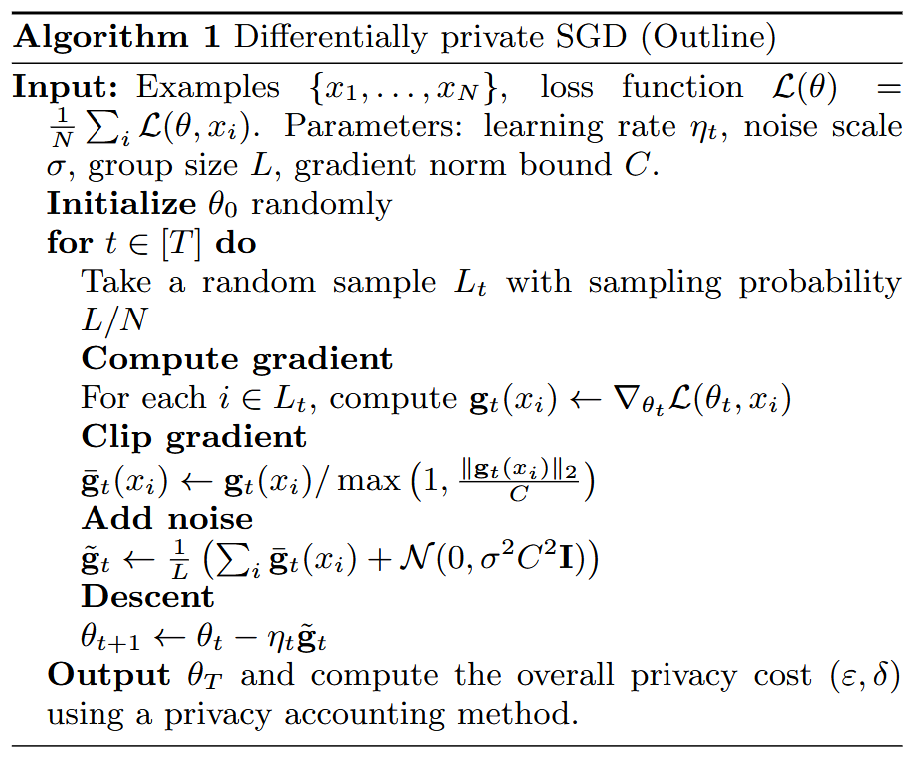
\includegraphics[width=\linewidth]{img/DP_SGD_pseudocode}
		\caption{\ac{DP-SGD} pseudocode as published by Abadi et al.~\cite{abadi2016deep}.}
		\label{fig:dpsgdpseudocode}
	\end{figure}
	
	\subsubsection{Central vs.\ Local \ac{DP} in FL}
	
	In central DP, the server adds noise after aggregating the client updates. This setting assumes a trusted aggregator while protecting the aggregated updates before they are shared with third parties.
	
	In the considered setting, client updates must be protected against inference attacks by the aggregator or adversaries eavesdropping on the client--server communication, requiring local \ac{DP}. To achieve this, each client adds noise to its update before transmission. Since the noise added by individual clients accumulates during aggregation, local \ac{DP} requires a higher effective noise magnitude and therefore incurs a greater loss in accuracy.
	
	\subsection{Robustness: Byzantine-Tolerant Aggregation}
	This section introduces the Byzantine fault model and presents two aggregation schemes designed to mitigate the effects of Byzantine adversaries.
	
	\subsubsection{Byzantine Fault Model}
	Byzantine Fault Tolerance is a property of a distributed system that allows for the system to stay operational while some components fail or act maliciously.
	
	A $\eta$-fraction Byzantine adversary means that $\eta$\% of the clients are acting maliciously. In the conducted experiments, malicious behavior means communicating manipulated gradients to poison the central model, e.g. insert a backdoor, degrade the general performance or enable label flipping attacks.
	
	\subsubsection{Krum}
	
	Krum~\cite{Krum}, proposed by Blanchard et al. in 2017, enhances robustness to Byzantine adversaries by selecting updates closest to their XX neighbors, effectively focusing on the densest cluster of updates of size XX. This ensures the training process is provably Byzantine-tolerant but relies on the assumption that honest updates cluster together, which only holds when data distributions across clients are similar. Under data heterogeneity, this assumption breaks down, leading to performance degradation because honest updates may be discarded if they deviate significantly from the majority.
	
	\subsubsection{FLTrust}
	
	FLTrust~\cite{cao2021fltrust} was introduced by Cao et al. in 2020 and mitigates malicious updates through trust scores. These are obtained by calculating the cosine similarity of the local update to an update anchor computed on a small root dataset held by the server. The method relies on the assumption that the server has access to a dataset representing the general data distribution across all clients.
	
	\subsection{Performance: Communication Efficiency}
	Another practical limitation especially in mobile applications is the available bandwidth to transmit local updates to the aggregator. We therefore include a method to communicate sparse instead of dense updates.
	
	\subsubsection{Top-$k$ Gradient Sparsification}
	
	Top-$k$ gradient sparsification~\cite{aji2017topk} reduces communication during gradient transmission by retaining only the $k$ largest gradient components, where $k$ is a fixed fraction of the model dimension $d$.
	
	Discarding the remaining gradient components inevitably results in information loss, leading to reduced model performance. The extent of this degradation depends on how the optimization information is distributed across the gradient, with models relying on a small number of dominant components generally being less affected than those requiring information from many dimensions.
	
	\subsubsection{Relation to Model Dimensionality}
	
	The term $d/(\epsilon^2 n)$ in the theoretical lower bound~\cite{allouah2023trilemma} raises the assumption that //TODO
	
	\subsection{The Privacy--Robustness--Performance Trilemma}
	This section first presents the theoretical lower bound of the trilemma and then discusses its implications for empirical evaluation, motivating efficiency as a fundamental third axis.
		
	\subsubsection{Theoretical Lower Bound}
	
	Allouah et al.~\cite{allouah2023trilemma} proved that any algorithm simultaneously guaranteeing $\epsilon$-local DP and robustness against an $\eta$-fraction Byzantine adversary incurs a mean estimation error of at least
	\begin{equation}
	\Omega!\left(\frac{\eta}{\epsilon^2} + \frac{d}{\epsilon^2 n} + \eta G^2\right).
	\label{lowerBoundTheory}
	\end{equation}
	This lower bound establishes that the costs of privacy and Byzantine robustness are fundamentally coupled. In particular, the cross-term $\eta/\epsilon^2$ shows that these costs interact multiplicatively rather than additively.
	
	\subsubsection{Efficiency Axis Extension}
	
	The same authors proposed the aggregation schemes SMEA and CAF, which match this theoretical lower bound. However, both methods incur a runtime complexity that scales cubically with the model dimension, rendering them impractical for large-scale models. Furthermore, the runtime of SMEA grows exponentially with the number of tolerated Byzantine adversaries, making it infeasible in realistic federated learning settings.
	
	The term $\frac{d}{\varepsilon^2 n}$ in \ref{lowerBoundTheory} further relates the model dimension $d$ to the communication cost and achievable estimation error. Consequently, maintaining accuracy for high-dimensional models requires either relaxing privacy guarantees or integrating a larger number of participating clients.
	
	
	\subsubsection{Empirical Evidence of Compounding}
	
	In 2021, Guerraoui et al. empirically investigated the question \textit{"Differential Privacy and Byzantine Resilience in SGD: Do They Add Up?"}~\cite{guerraoui2021differentialprivacybyzantineresilience}. They showed that a naive combination of privacy- and robustness-enhancing methods, namely \ac{DP-SGD} and Minimum-Diameter Averaging (MDA)~\cite{elmhamdi2020genuinelydistributedbyzantinemachine}, leads to unfavorable scaling with the model dimensionality and super-additive performance degradation. These findings support the theoretical results of Allouah et al. and reinforce the need to treat efficiency as a fundamental third axis in future experimental studies.

	
	% --------------------------------------------------
	\section{Threat Model and Metrics}
	\label{sec:threat}
	% --------------------------------------------------
	This chapter maps out the assumed threat model and introduces the metrics used to evaluate the three axes.
	
	\subsection{Threat Model}
	
	We assume an honest-but-curious central server that adheres to protocol specifications but may attempt to infer private information from transmitted updates, motivating the use of differential privacy (DP) to safeguard client data. The adversary is characterized by a fraction $\eta$ of malicious clients, capable of arbitrarily manipulating gradients (e.g., through label-flipping attacks, as formalized in Fang et al.~\cite{fang2020poisoning}). These clients aim to corrupt the global model by injecting adversarial updates. Crucially, we assume no collusion between Byzantine clients and the server, restricting adversarial behavior to local manipulations of gradients. This assumption simplifies the analysis while maintaining practical relevance for decentralized learning systems.
	
	\subsection{Evaluation Metrics}
	\label{sec:metrics}
	
	As suggested by Allouah et al.~\cite{allouah2023balancing}, every configuration is evaluated simultaneously across all three trilemma axes:
	
	\paragraph{Privacy.}
	
	The privacy objective is quantified by the accumulated $(\epsilon,\delta)$-differential privacy (DP) budget after $T$ rounds, tracked using the Rényi accountant~\cite{mironov2019rényi}. Additionally, the vulnerability to membership inference attacks is assessed by measuring the success rate of such attacks against a shadow model baseline~\cite{song2019membership}.
	
	\paragraph{Robustness.}
	
	Robustness is evaluated by the attack success rate (ASR) under label-flipping attacks and the accuracy gap $\Delta_{acc}$ relative to a clean FedAvg baseline. The accuracy gap captures untargeted performance degradation caused by adversarial clients, providing a measure of resilience to Byzantine behavior.
	
	\paragraph{Performance.}

	The performance metric includes test accuracy on held-out data, communication cost (bytes sent per client per round), and wall-clock training time. These metrics collectively assess the trade-off between model utility, resource efficiency, and computational feasibility in decentralized learning systems.
	
	\subsection{Trilemma Visualization}
	
	\placeholder{%
		Radar / simplex chart positioning each of the 8 configurations relative to the
		three axes, analogous to Figure~1 of~\cite{allouah2023balancing}.
		Include actual figure once results are available.%
	}
	
	% --------------------------------------------------
	\section{Methods}
	\label{sec:method}
	% --------------------------------------------------
	This section briefly describes and justifies the selected methods for each axis.
	\subsection{Baseline: FedAvg}
	
	\placeholder{%
		Standard weighted average aggregation~\cite{mcmahan2017fedavg};
		serves as the reference point for all accuracy gaps;
		no privacy, robustness, or compression applied.%
	}
	
	FedAvg, introduced by McMahan et al. in 2017~\cite{mcmahan2017fedavg}, is a widely used aggregation strategy in \ac{FL} designed to handle non-\ac{IID} data efficiently. It computes a weighted average of local model updates, with weights determined by the size of each client’s local dataset. The paper establishes baselines on standard datasets such as MNIST and CIFAR-10, making FedAvg a foundational reference for evaluating \ac{FL} methods. Its simplicity and effectiveness in early \ac{FL} research have cemented its role as a standard baseline for comparative studies.
	
	\subsection{Privacy Mechanism: \ac{DP-SGD}}
	
	\placeholder{%
		Per-sample clipping norm $C$; noise multiplier $\sigma$; privacy budget
		$\epsilon \in \{1, 5, 10\}$, $\delta = 10^{-5}$;
	}
	
	\subsection{Robustness Mechanism: FLTrust}
	
	\placeholder{%
		Server root dataset construction; trust score computation;
		cosine similarity clipping; parameter: root dataset size;
	}
	
	The root dataset for the central server was obtained by randomly sampling a parametrized number of data points, uniformly distributed over all classes, from the training set.
	
	The trust score for weighting the local contributions is calculated as the cosine similarity to the update vector that was computed from the root data set as depicted in figure \ref{fig:fltrustupdate}.
	\begin{figure*}[h!]
		\centering
		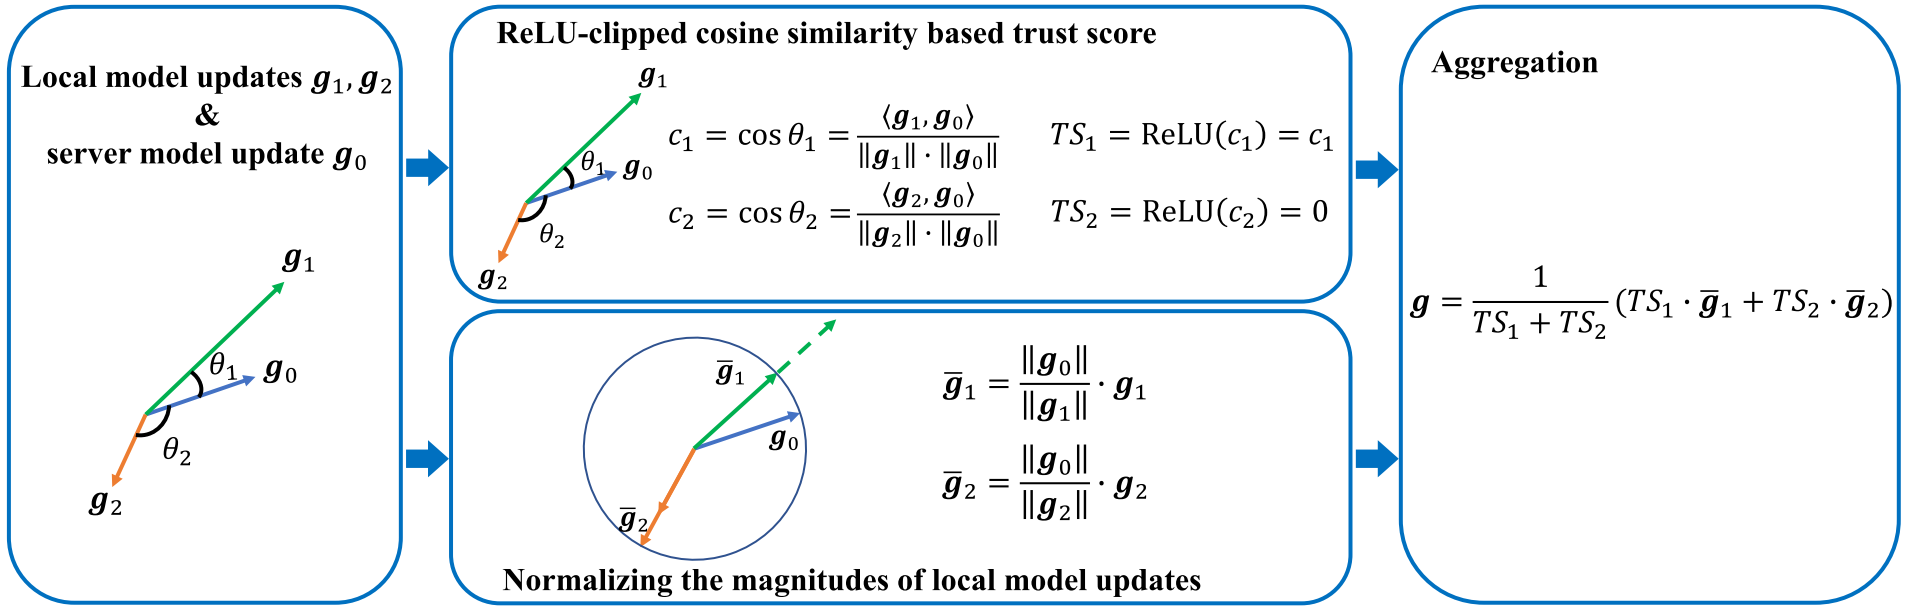
\includegraphics[width=\textwidth]{img/fltrust_update}
		\caption{Global aggregation rule for FLTrust as introduced by Cao et al.~\cite{cao2021fltrust}.}
		\label{fig:fltrustupdate}
	\end{figure*}
	
\subsection{Performance Mechanism: Top-$k$ Sparsification}
	
	\placeholder{%
		Fraction $k \in \{1\%, 10\%\}$ of $d$ transmitted per round;
		error feedback accumulator;
		custom Flower strategy wrapper;
		interaction with gradient clipping discussed in Section~\ref{sec:interaction}.%
	}
	
	
\subsection{Mechanism Interaction Effects}
	\label{sec:interaction}
	
	\placeholder{%
		Theoretical analysis of how clipping (DP) and cosine-similarity clipping
		(FLTrust) may amplify each other; how sparsification changes the effective
		gradient distribution seen by the aggregator;
		hypothesis: super-additive cost for the full combination.%
	}
	
	% --------------------------------------------------
	\section{Experimental Setup}
	\label{sec:setup}
	% --------------------------------------------------
	
	\subsection{Experimental Grid}
	The experimental grid is described in table \ref{table:grid}.
	
	\begin{table}[h]
		\centering
		\begin{tabular}{llll}
			\hline
			\rowcolor[HTML]{C0C0C0} 
			\textbf{Identifier} & \ac{DP-SGD} & FLTrust & Top-k \\ \hline
			Base &  &  &  \\ \hline
			\rowcolor[HTML]{EFEFEF} 
			DP & \multicolumn{1}{c}{\cellcolor[HTML]{EFEFEF}x} &  &  \\ \hline
			FLTrust &  & \multicolumn{1}{c}{x} &  \\ \hline
			\rowcolor[HTML]{EFEFEF} 
			TOPK &  &  & \multicolumn{1}{c}{\cellcolor[HTML]{EFEFEF}x} \\ \hline
			DP+FLTrust & \multicolumn{1}{c}{x} & \multicolumn{1}{c}{x} &  \\ \hline
			\rowcolor[HTML]{EFEFEF} 
			DP+TOPK & \multicolumn{1}{c}{\cellcolor[HTML]{EFEFEF}x} &  & \multicolumn{1}{c}{\cellcolor[HTML]{EFEFEF}x} \\ \hline
			FLTrust+TOPK &  & \multicolumn{1}{c}{x} & \multicolumn{1}{c}{x} \\ \hline
			\rowcolor[HTML]{EFEFEF} 
			ALL & \multicolumn{1}{c}{\cellcolor[HTML]{EFEFEF}x} & \multicolumn{1}{c}{\cellcolor[HTML]{EFEFEF}x} & \multicolumn{1}{c}{\cellcolor[HTML]{EFEFEF}x} \\ \hline
		\end{tabular}
		\caption{Identifiers and applied methods for the different experimental setups.}
		\label{table:grid}
	\end{table}
	

	\subsection{Datasets}

	\paragraph{MNIST.} The MNIST dataset consists of 70,000 grayscale images of handwritten digits with a resolution of 28 × 28 pixels, each labelled with the corresponding digit in the range [0,9]. It is divided into a training set of 60,000 samples and a test set of 10,000 samples. Owing to its simplicity, the dataset is widely used to benchmark image classification models and verify their functionality before extending them to more complex datasets.
	
	\paragraph{CIFAR-10.} CIFAR-10 is a benchmark dataset for object classification comprising 60,000 RGB images with a resolution of 32 × 32 pixels, categorized into 10 classes. It is divided into 50,000 training samples and 10,000 test samples and is widely used for training and benchmarking object classification networks.
	
	
	\subsection{Hyperparameters}
	
	\placeholder{%
		Justify each choice with respect to BLADES baselines.%
	}
	\paragraph{Static.}
	seed, attack type
	
	\paragraph{Dynamic.}
	Number of clients, number of rounds, byzantine fraction, root dataset size, attack scale, epsilon, top-k fraction
	\subsection{Software Stack}
	
	\begin{itemize}
		\item \textbf{Flower} (flwr)~\cite{beutel2020flower} --- \ac{FL} orchestration,
		client/server simulation, strategy interface.
		\item \textbf{Opacus}~\cite{yousefpour2021opacus} --- \ac{DP-SGD}, Rényi \ac{DP}
		accounting, gradient clipping.
		\item \textbf{FLTrust}~\cite{cao2021fltrust} --- FLTrust defense implementation.
		\item \textbf{Custom} --- Top-$k$ gradient sparsification wrapper.
	\end{itemize}
	
	\placeholder{%
		Software versions; hardware (GPU/CPU); random seed management; number of
		independent runs per configuration.%
	}
	
	\subsection{Reproducibility}
	
	\placeholder{%
		Pointer to open-source repository; instructions to replicate all 8 configurations;
		fixed random seeds; containerization (Docker/Conda environment file).%
	}
	
	% --------------------------------------------------
	\section{Results}
	\label{sec:results}
	% --------------------------------------------------
	
	\subsection{Baseline Reproduction (RQ1 -- Sanity Check)}
	
	\placeholder{%
		FedAvg and FLTrust baselines on MNIST vs.\ published BLADES numbers;
		table: our accuracy / ASR vs.\ reported values; discussion of any deviations.%
	}
	
	\subsection{Isolation: Individual Mechanism Costs (RQ1)}
	
	\placeholder{%
		One subsection or figure per mechanism;
		accuracy vs.\ $\epsilon$ curve for DP-SGD;
		ASR vs.\ $\eta$ for FLTrust;
		accuracy / bytes trade-off for Top-$k$ at $k \in \{1\%, 10\%\}$;
		results on both MNIST and CIFAR-10.%
	}
	
	\subsubsection{\ac{DP-SGD} Cost}
	\placeholder{Accuracy curves for $\epsilon \in \{1,5,10\}$; privacy budget consumed.}
	
	\subsubsection{FLTrust Cost}
	\placeholder{Accuracy gap and ASR for varying Byzantine fractions.}
	
	\subsubsection{Top-$k$ Sparsification Cost}
	\placeholder{Accuracy, bytes per round, and wall-clock time for $k \in \{1\%,10\%\}$.}
	
	\subsection{Combination: Pairwise and Full Interactions (RQ2)}
	
	\placeholder{%
		Main results table: 8 configurations $\times$ all metrics;
		additive vs.\ super-additive cost analysis;
		focus on \ac{DP}+FLTrust interaction;
		radar / simplex visualization (Figure~\placeholder{X}).%
	}
	
	\subsubsection{\ac{DP} + Robustness}
	\placeholder{Effect on accuracy and ASR; comparison to individual costs.}
	
	\subsubsection{\ac{DP} + Compression}
	\placeholder{Effect on accuracy and communication cost; interaction with noise.}
	
	\subsubsection{Robustness + Compression}
	\placeholder{Effect on ASR and bytes per round.}
	
	\subsubsection{Full Combination (\ac{DP} + Robustness + Compression)}
	\placeholder{Worst-case configuration; super-additive compounding quantified.}
	
	\subsection{MNIST vs.\ CIFAR-10 Comparison}
	
	\placeholder{%
		How results scale with dataset complexity;
		does the compounding pattern hold across both?%
	}
	
	% --------------------------------------------------
	\section{Discussion}
	\label{sec:discussion}
	% --------------------------------------------------
	
	\subsection{Interpretation of Compounding Effects}
	
	\placeholder{%
		Relate empirical findings to the theoretical cross-term $\eta/\epsilon^2$;
		characterize compounding as additive / sub-additive / super-additive per
		configuration pair; intuition for why DP clipping and FLTrust cosine clipping
		interact destructively.%
	}
	
	\subsection{Mitigation: Joint Clipping-Norm Calibration (RQ3)}
	
	\placeholder{%
		Heuristic: jointly set DP clipping norm $C$ and FLTrust trust threshold to
		minimize redundant gradient suppression;
		description of the calibration procedure;
		results vs.\ uncalibrated worst-case combination;
		formal guarantee preservation argument.%
	}
	
	\subsection{Practical Recommendations}
	
	\placeholder{%
		When to prioritize which axis;
		safe operating region in the trilemma space;
		guidance on $(\epsilon,k)$ parameter selection given a robustness requirement.%
	}
	
	% --------------------------------------------------
	\section{Limitations and Future Work}
	\label{sec:limitations}
	% --------------------------------------------------
	
	\subsection{Limitations}
	
	\placeholder{%
		Single attack type (label-flipping); single aggregation rule (FLTrust);
		membership inference approximation (shadow model only);
		limited $\epsilon$ grid; MNIST/CIFAR-10 may not represent medical/financial FL.%
	}
	
	The experiments in this project were conducted under several simplifications to provide a lightweight anchor for future research. 
	\paragraph{Simple models and datasets.}
	The datasets and models selected offer good comparability with existing work but may not fully represent the data analyzed in practical \ac{FL} applications (e.g., financial or medical domains) or complex architectures (e.g., transformer-like models). 
	
	\paragraph{Limited method coverage.} We evaluated only a single method and at most one attack type per axis. The baseline for membership inference attack success rate was approximated using a shadow model, and the privacy budget was constrained to a limited $\varepsilon$-grid to balance computational feasibility with analytical rigor. 
	
	\paragraph{Privacy budget schedule.} The privacy budget was spent uniformly over time, but recent research by Kiani et al.~\cite{kiani2025differentiallyprivatefederatedlearning} suggests that a time-adaptive approach yields better privacy-utility-tradeoffs.
	
	\paragraph{Stateless Clients.} The clients do not preserve a state over multiple rounds. In combination with top-k sparsification, this hinders small but repeated updates to accumulate to meaningful contributions over time. Introducing a client state requires well-behaved clients to correctly maintain the state and stay synchronized with the central model, which is realistic for distributed training but not a reasonable assumption in federated learning. Another option is to share the state with the central server, defeating the purpose of the sparsification and introducing new privacy vulnerabilities.
	
	\subsection{Future Work}
	
	\placeholder{%
		Extend to Krum, SMEA, CAF aggregators;
		stronger attacks (model poisoning~\cite{fang2020poisoning});
		LoRA+DP reparametrization~\cite{liu2025dplora} for the efficiency axis;
		theoretical tightness of joint calibration heuristic.%
	}
	
	Future work should aim to expand the experimental setup to encompass a broader range of methods (e.g., Krum, SMEA, CAF for aggregation) and evaluate stronger adversarial scenarios, such as model poisoning attacks described by Fang et al.\cite{fang2020poisoning}. Additionally, exploring reparametrization techniques such as the Low-Rank-adaptation method proposed by Liu et al.\cite{liu2025dplora} could provide insights into balancing efficiency and privacy in \ac{FL} systems. 
	
	Other promising directions include varying the Byzantine fraction, testing alternative threat models (e.g., malicious servers, collusion between malicious clients and servers), or introducing data heterogeneity through artificially distributed datasets. These extensions would better reflect real-world complexities and enable more robust comparisons across methodologies..
	
	% --------------------------------------------------
	\section{Conclusion}
	\label{sec:conclusion}
	% --------------------------------------------------
	
	\placeholder{%
		Restate research questions and answers;
		key quantitative finding (e.g.\ full combination degrades accuracy by $X$\% beyond
		sum of individual costs);
		mitigation heuristic reduces compounding by $Y$\% without formal guarantee loss;
		open-source pipeline as contribution to the community.%
	}
	
	% --------------------------------------------------
	% References
	% --------------------------------------------------
	\bibliographystyle{IEEEtran}
	\bibliography{bib.bib}
	
	\section{APPENDIX}
	
	\begin{figure}
		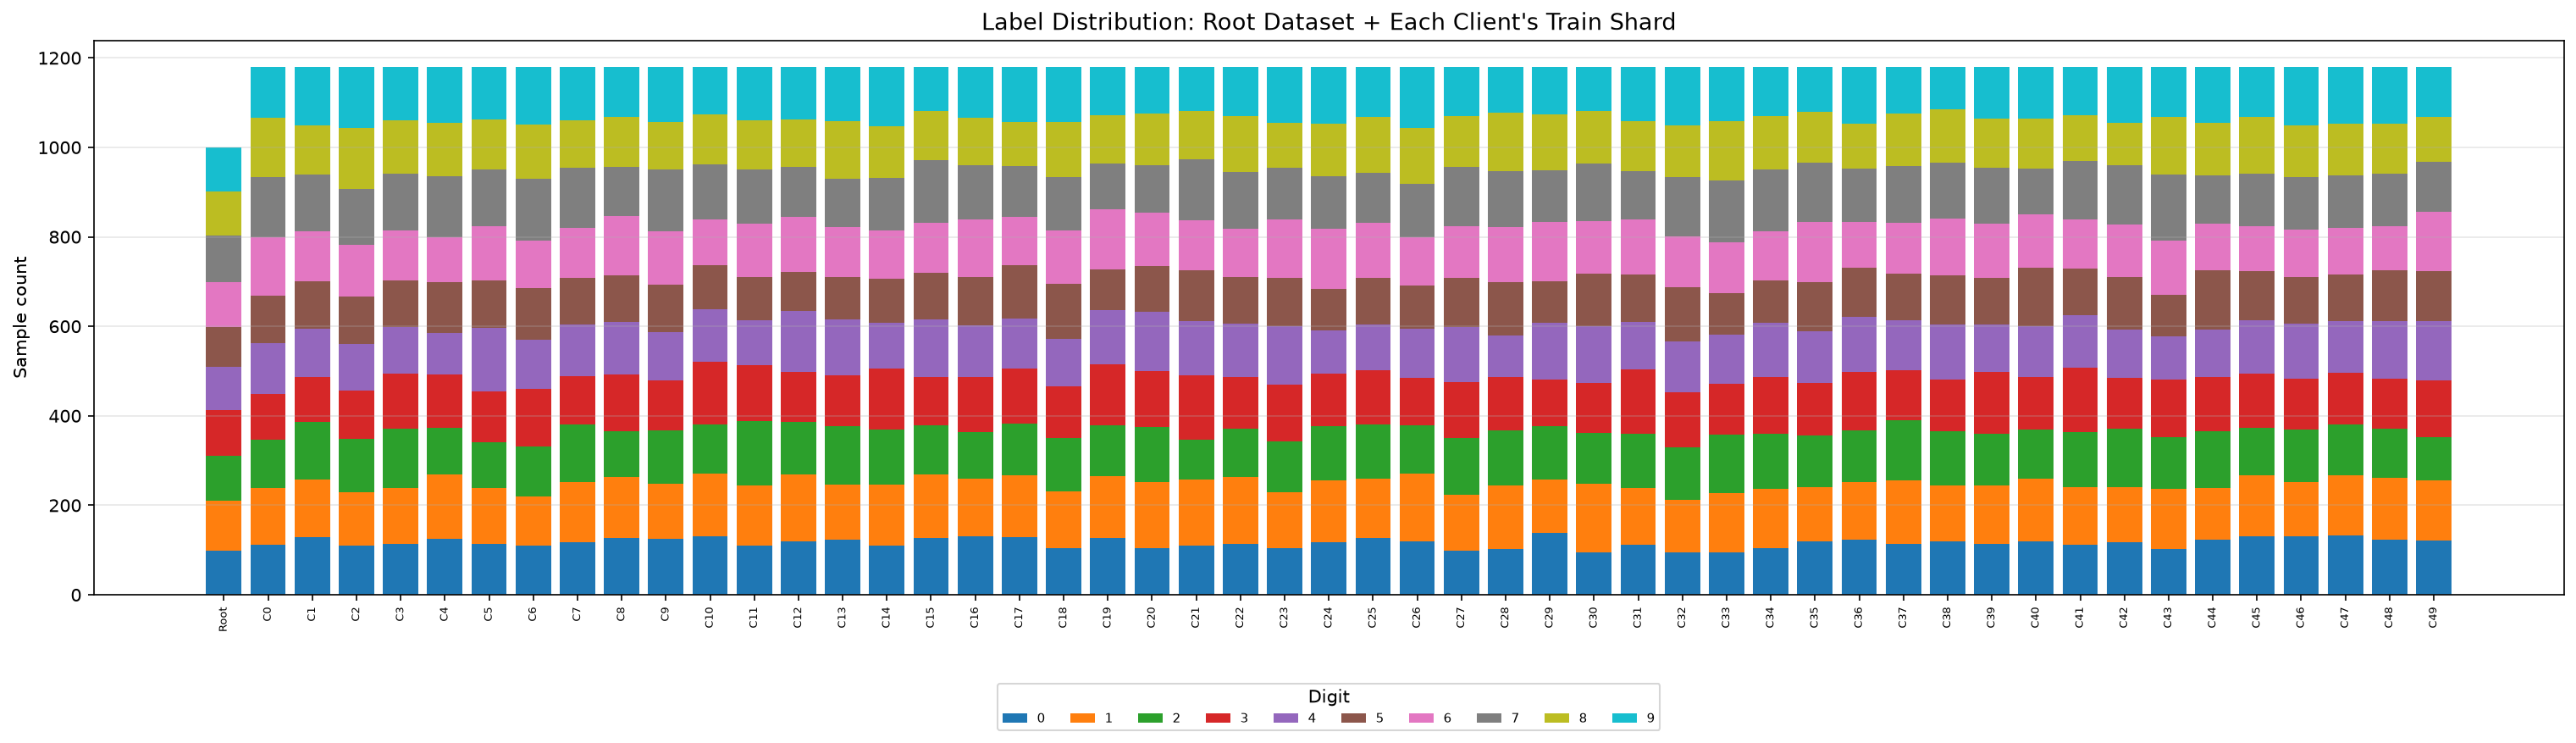
\includegraphics{img/MNIST_07-10/label_distribution.png}
		\label{fig:labeldistr}
	\end{figure}
\end{document}